\documentclass{article}
\usepackage{qilin}
\title{ECE159 Notes}
\author{QiLin Xue}
\lhead{ECE159}
\rhead{QiLin Xue}
\renewcommand{\qedsymbol}{
\includegraphics[height=3ex]{kalda.png}}

\newcommand{\equals}{=}

\begin{document}
    \maketitle
    % The following notes were compiled from several sources: The majority of the theory was taken from the lectures and textbook, although some parts were taken from Purcell and Morin's \textit{Electricity and Magnetism}, and the problems were taken from Jaan Kalda's \href{https://www.ioc.ee/~kalda/ipho/electricity-circuits.pdf}{handout} on electrical circuits (hence the funky notation). Solutions were written as part of a joint \href{https://physoly.tech/kalda/}{collaboration}. I do not claim originality of the problems or solutions, though I selected them to reflect the course.
    \tableofcontents
    % \section{Positionality}
\begin{itemize}
    \item A \textbf{position} defines your orientation with respect to an \textbf{entity}.
    \begin{idea}
        How does PIAA affect positionality?
    \end{idea}
    Some ideas from classmates:
    \begin{itemize}
        \item Perception sets initial opinion
        \item You interpret things based on your positionWhat or what you don't perceive affects your positionality.
        \item In breaking the action of perceive-act, you include steps that allow the time to assess your position.
        \item Filters (in perception) depend on position
        \item Understanding your position allows you to assess your interpretations
    \end{itemize}
    \item Subconcious \textbf{bias} will be brought to the table depending on your position, so others can explicityl see how \textit{you} are looking at a situation. 
\end{itemize}
    \section{DC circuit Analysis}
    \subsection{Voltage and Current Division}
    For a series circuit, we can calculate the equivalent resistance by adding them.
    \begin{center}
        \begin{tikzpicture}[transform shape, thick]
            \draw (0, 0) to [V, i_>=$i$,
                                l=$V$, invert] (0, 4)
                         to [R, l=$R_1$] (4, 4) node[right] {$A$}
                         to [R, l=$R_2$] (4, 0)
                         to node[ground]{} (0,0); 
            \draw[fill=black] (4,4) circle (1.5pt);
            \draw[fill=black] (4,0) circle (1.5pt);
        \end{tikzpicture}
    \end{center}
    For this circuit, we have:
    \begin{equation}
        R_\text{eq} = R_1 + R_2
    \end{equation}
    and the voltage:
    \begin{equation}
        V_A = \frac{R_2}{R_1+R_2}V
    \end{equation}
    \begin{proof}
        The current is given by $i = \frac{V}{R_1+R_2}$ and the voltage at $A$ is given by:
        \begin{equation}
            V_A = V - iR_1 = V\left(1 - \frac{R_1}{R_1+R_2}\right) = \frac{R_2}{R_1+R_2}V
        \end{equation}
    \end{proof}
    For a parallel circuit, the effective resistance is the harmonic sum:
    \begin{center}
        \begin{tikzpicture}[transform shape, thick, american currents]
        \draw (0, 0) to [V, i_>=$i$, l=$V$] (0, 4)
                     -- (4,4)
                     to [R,i_>=$i_1$, l=$R_1$] (4, 0)
                     -- (0,0);
        \draw (4,4) -- (8,4)
                    to [R, i_>=$i_2$, l=$R_2$] (8,0)
                    to node[ground]{} (0,0);
        \end{tikzpicture}
    \end{center}
    In this circuit, we have:
    \begin{equation}
        R_\text{eq} = \left(\frac{1}{R_1} + \frac{1}{R_2}\right)^{-1} = \frac{R_1R_2}{R_1+R_2}
    \end{equation}
    and the current in the branches is given by:
    \begin{equation}
        i_1 = \frac{R_2}{R_1+R_2}i
    \end{equation}
    \begin{proof}
        The voltage drop across $R_1$ and $R_2$ must be the same, so:
        \begin{equation}
            i_1R_1 = i_2R_2
        \end{equation}
        We also have $i_2=i-i_1$, which gives:
        \begin{equation}
            i_1R_1 = (i-i_1)R_2 \implies i_1 = \frac{R_2}{R_1+R_2}i
        \end{equation}
    \end{proof}
    \subsection{Mesh Analysis}
    In mesh analysis, Kirchoff's Voltage law $\sum V = 0$ is written for each independent loop, and a system of equation is solved. The number of independent loops can be determined by finding the minimum number of wire cuts needed such that there are no loops.
    \begin{center}
        \begin{tikzpicture}[transform shape, thick, american currents]
        \draw (-4, 0) to [V, i_>=$i$, l_=$V\equals 2\si{\volt}$, invert] (4, 0)
                     -- (4,3) -- (3.5, 3) -- (3.5, 4) to
                [R, l_=$R_2\equals3\si{\ohm}$, i=$i-i_1$] (0,4) node[above] {$a$} to
                [R, l_=$R_1\equals 2\si{\ohm}$, i=$i-i_1+i_2$] (-3.5, 4)
                -- (-3.5, 3) -- (-4, 3) to node[ground,rotate=-90]{} (-4,0);
        \draw (-3.5, 3) -- (-3.5, 2) to [R, l_=$R_4\equals 5\si{\ohm}$, i<=$i_1-i_2$] (0,2) node[below] {$b$} to [R, l_=$R_5\equals 1\si{\ohm}$, i<=$i_1$] (3.5, 2) -- (3.5, 3);
        \draw (0, 4) to [R, l_=$R_3\equals 4\si{\ohm}$] (0,2);
        \draw (-2.5,3) node[scale=3]{$\circlearrowleft$} node{$A$};
        \draw (2,3) node[scale=3]{$\circlearrowleft$} node{$B$};
        \draw (0,1) node[scale=3]{$\circlearrowleft$} node{$C$};
        \end{tikzpicture}
    \end{center}
    We have three independent loops, labelled as $A,B,C$, which gives the system of three equations:
    \begin{align}
        0 &= -i_2R_3-(i-i_1+i_2)R_1+(i_1-i_2)R_4 \\ 
        0 &= -(i-i_1)R_2 + i_2R_3 + i_1R_5 \\ 
        0 &= V - i_1R_5 - (i_1-i_2)R_4
    \end{align}
    Solving this system gives:
    \begin{equation}
        (i, i_1, i_2) =\left(-\frac{144}{181}\si{A}, \frac{82}{181}\si{A}, \frac{26}{181}\si{A}\right)
    \end{equation}
    which can be used to determine the currents in all resistors and the associated voltages.
    \subsection{Nodal Analysis}
    In nodal analysis, we deal with the potentials at each node and write out Kirchoff's current law $\sum I = 0$ for the current \textit{leaving} (or alternatively, entering) each node for each node where the potential is unknown. Let the nodes labelled $a$ and $b$ have potentials $V_a$ and $V_b$. Then we have:
    \begin{align}
        0 &= \frac{V_a-V}{R_2} + \frac{V_a-V_b}{R_3} + \frac{V_a-0}{R_1} \\
        0 &= \frac{V_b-V}{R_5} + \frac{V_b-V_a}{R_3} + \frac{V_b-0}{R_4} 
    \end{align}
    which after solving, gives:
    \begin{equation}
        (V_a, V_b) = \left(\frac{176}{181}\si{V}, \frac{280}{181}\si{V}\right)
    \end{equation}
    which can be easily confirmed via the mesh analysis done above.
    \subsection{Superposition}
    Kirchoff's equations are linear. Each term includes only a first power of a current or a voltage, hence we can apply superposition. Let there be $n$ independent voltage sources and $m$ independent current sources. The current in the $j^\text{th}$ wire can be found as:
    \begin{equation}
        I_j = \sum_{k=1}^{n+m} I_j(k)
    \end{equation}
    where $I_j(k)$ is the current in that wire when only the $k^\text{th}$ battery (or current source) is included into the circuit. All other batteries are short circuited and all other current sources are removed by cutting off a connection wire.
    \begin{example}
        In the following circuit, we have $\mathcal{E}_1=\mathcal{E}_2$ and all the resistors are equal: $R_1=R_2=R_3=R_4=R$. Let us attempt to find the current through each resistor.
        \begin{center}
            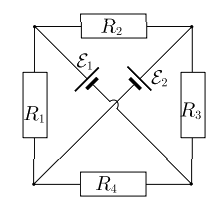
\includegraphics[width=0.3\linewidth]{estpho2012.png}
        \end{center}
        We make use of the superposition principle and start by short-circuiting $\mathcal{E}_2$. This leads to the following equivalent circuit:
    \begin{center}
        \begin{tikzpicture}[transform shape, thick]
        \ctikzset{bipoles/thickness=2}
        \ctikzset{label/align = smart}
        \coordinate  (A) at (0,0);
        \coordinate  (B) at (3,0);
        \coordinate  (C) at (6,0);
        \coordinate  (D) at (9,0);
        
        \draw (B) to [battery1, l=$\mathcal{E}_1$] (C) to ($(C) + (0,1)$) to [R, l=$R_3$] ($(D) + (0,1)$) to ($(D) + (0,-2)$) to ($(A) + (0,-2)$) to ($(A) + (0,1)$) to [R, l=$R_1$] ($(B) + (0,1)$) to (B);
        
        \draw ($(A) + (0,-1)$) to [R, l=$R_2$] ($(B) + (0,-1)$) to (B);
        \draw (C) to ($(C) + (0,-1)$) to [R, l=$R_4$] ($(D) + (0,-1)$);
        \end{tikzpicture}
        \end{center}
        Since all resistors have a resistance of $R$, this leads to the following currents in each resistor (going back to the original diagram):
        \begin{align*}
            R_1 &\rightarrow \frac{\mathcal{E}}{2R} \, \text{(downwards)} \\ 
            R_2 &\rightarrow \frac{\mathcal{E}}{2R} \, \text{(rightwards)} \\ 
            R_3 &\rightarrow \frac{\mathcal{E}}{2R} \, \text{(downwards)} \\
            R_4 &\rightarrow \frac{\mathcal{E}}{2R} \, \text{(leftwards)}
        \end{align*}
        and similarly if we short $\mathcal{E}_1$, we get the following currents:
        \begin{align*}
            R_1 &\rightarrow \frac{\mathcal{E}}{2R} \, \text{(downwards)} \\ 
            R_2 &\rightarrow \frac{\mathcal{E}}{2R} \, \text{(leftwards)} \\ 
            R_3 &\rightarrow \frac{\mathcal{E}}{2R} \, \text{(downwards)} \\
            R_4 &\rightarrow \frac{\mathcal{E}}{2R} \, \text{(rightwards)}
        \end{align*}
        By considering the superposition of these currents, we get after adding them together:
        \begin{align*}
            R_1 &\rightarrow \frac{\mathcal{E}}{R} \, \text{(downwards)} \\ 
            R_2 &\rightarrow 0 \\ 
            R_3 &\rightarrow \frac{\mathcal{E}}{R} \, \text{(downwards)} \\
            R_4 &\rightarrow 0
        \end{align*}
        Alternatively we can solve this problem via symmetry. Note that there is reflection symmetry across the vertical line. This means that the current does not have a preferred direction of going either right or left, so that the current in $R_2$ and $R_4$ will be zero. As a result, we can simply replace these two resistors with an open gap, which results in the other four circuit elements in series:
        $$    I = \frac{2\mathcal{E}}{2R} = \frac{\mathcal{E}}{R}
        $$
        which travels in a ``zigzag'' pattern.
    \end{example}
    
    \subsection{Source Transformation}
    A source transformation is the process of replacing a voltage source $v_s$ in series with a resistor $R$ by a current source $i_s$ in parallel with a resistor $R$, or vice versa. For example, these two circuits are equivalent:
    \begin{center}
        \begin{tikzpicture}[transform shape, thick]
            \draw (3,0) node[right] {$b$} -- (0, 0) to [V,
                                l=$v_s$, invert] (0, 2)
                         to [R, l=$R$] (3, 2) node[right] {$a$}; 
        \end{tikzpicture}
        \begin{tikzpicture}[transform shape, thick, american currents]
            \draw (3,0) node[right] {$b$} -- (0, 0) to [I,
                                l=$i_s$] (0, 2)
                         -- (3, 2) node[right] {$a$}; 
            \draw (1.5,0) to [R, l_=$R$] (1.5, 2);
        \end{tikzpicture}
    \end{center}
    where $v_s=i_sR$.
    \begin{proof}
        We can show that this is valid by letting $V_a=V$ and $V_b=0$. and calculating the current at $a$. For the first circuit, we have:
        \begin{equation}
            i = \frac{v_s-V}{R}
        \end{equation}
        For the second circuit, the current through the resistor is $i_R = \frac{V}{R}$ (downwards) and letting $i_s = \frac{v_s}{R}$ we have the current at $a$ as:
        \begin{equation}
            i = \frac{v_s}{R} - \frac{V}{R}
        \end{equation}
        which we see is the same for both cases.
    \end{proof}
    \begin{example}
        Suppose we have $n$ batteries with a voltage of $\mathcal{E}_i$ and internal resistances of $r_i$ with $i=1,2,\dots,n$, all connected in parallel. What is the effective electromotive force and the internal resistance of such a system of batteries?
        \vspace{2mm}

        We treat the batteries as $n$ current sources providing a current of $I_i = \dfrac{\mathcal{E}_i}{r_i}$. When determining an equivalent circuit, all the current sources add up to a total current of:
$$I_\text{total} = \sum_{i=1}^n \frac{\mathcal{E}_i}{r_i}$$and applying the idea again, this is equivalent to an effective voltage source of $\mathcal{E}_\text{eff} = I_\text{total}R_\text{eff}$ with the effective resistance being:
$$R_\text{eff} = \left(\sum_{i=1}^nr_i^{-1}\right)^{-1}$$since we are adding resistors in parallel. Putting everything together gives:
$$\mathcal{E}_\text{eff} = \left(\sum_{i=1}^nr_i^{-1}\right)^{-1}\sum_{i=1}^n \frac{\mathcal{E}_i}{r_i}$$
\end{example}
\subsection{Thevenin Equivalent Circuit}
Thevenin's Theorem tells us that any two-terminal circuit can be replaced by an equivalent voltage source $V_\text{th}$ in series with a resistor $R_\text{th}$. These are related via:
\begin{equation}
    \label{thevenin}
    R_\text{th} = \frac{V_\text{th}}{I_\text{sc}}
\end{equation} 
To calculate $V_\text{th}$, we find the \textit{open circuit} voltage between the two terminals. To calculate $R_\text{th}$, there are two options:
\begin{enumerate}
    \item Remove all independent voltage and current sources and calculate the equivalent resistance across the terminals.
    \item Connect the two terminals via a wire with negligible resistance. Calculate the current $I_\text{sc}$ through this wire and we can calculate $R_\text{th}$ using equation \ref{thevenin}.
\end{enumerate}
\begin{example}
    Take the following circuit. What is the maximal power which can be dissipated on a load connected to the leads of the circuit?
    \begin{center}
        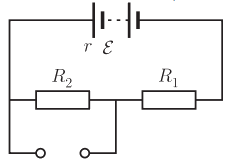
\includegraphics[width=0.3\linewidth]{pr10.png}
    \end{center}
    Recall that any circuit which consists of only resistors and batteries and has two ports $A$ and $B$ is equivalent to a series connection of a battery and a resistance. In other words, we consider the Thevenin equivalent of the circuit. The equivalent internal resistance can be found easily replacing the battery by a wire and using series and parallel connections.
$$R_{\text{eq}} = \frac{R_2(R_1+r)}{R_2 + (R_1+r)}$$The equivalent emf $\mathcal{E}_{\text{eq}}$ is the potential drop across $R_2$. The net resistance about the battery is $R_2 + (R_1+r)$, so the current through the battery is ,
\[ I = \mathcal{E}/r\implies I = \frac{\mathcal{E}}{R_1+R_2+r}.\]The potential drop about $R_2$ is then
\[V = IR_2 = \mathcal{E}\frac{R_2}{R_1+R_2+r}.\]This means that entire circuit in the figure can be substituted with an equivalent battery with
$$\mathcal{E}_{\text{eq}} = \mathcal{E}\frac{R_2}{R_1+R_2+r}.$$By the maximal power transfer theorem, this means that the resistance of the load attached needs to be $R=R_\text{eq}$. The potential drop across it is $\frac{\mathcal{E}}{2}$, so we have: 
\begin{align*}
P_{\text{max}} = \frac{\mathcal{E}_{\text{eq}}^2}{4R_{\text{eq}}} &= \frac{1}{4}\mathcal{E}^2 \left(\frac{R_2}{R_1+R_2+r}\right)^2 \cdot \frac{R_2 + (R_1+r)}{R_2\times (R_1+r)} \\
&= \frac{1}{4}\frac{R_2}{(r + R_1 + R_2)(R_1 + r)}\mathcal{E}^2
\end{align*}
\end{example}
\section{Operational Amplifiers}
An operational amplifier (op amp) is an active circuit element designed to perform mathematical operations of addition, subtraction, multiplication, division, differentiation, and integration.
\begin{center}
    \begin{circuitikz}[line width=1pt]
        \draw
        (0,0) node[op amp,yscale=1](opamp){} 
        (opamp.+) to[short, -o] ++(-.5,0) node[left]{$v_2$}
        (opamp.-) to[short, -o] ++ (-.5,0) node[left]{$v_1$}
        (opamp.out) to[short, -o] ++ (.5,0) node[right]{$v_0$}
        ;
    \end{circuitikz}
    
\end{center}
It is equivalent to the following circuit:
\begin{center}
    \begin{tikzpicture}[transform shape, thick]
        \draw  (-2,2) to [short, -o] (-2,2) node[left] {$v_1$} -- (0, 2) to [R, l=$R_i$, v_<=$v_d$] (0,-2) to [short, -o] (-2,-2) node[left] {$v_2$};

        \draw (6,0) node[right] {$v_0$} to [short, -o] (6,0) to [R, l=$R_0$] (3,0) to [V, l_=$A(v_2-v_1)$] (3, -1.5) node[ground]{};
    \end{tikzpicture}
\end{center}
where $A \gg 1$ is known as the open-loop voltage gain. The input resistance $R_i$ is typically very big.
\subsection{Ideal OP Amp}
For an ideal OP Amp, we have an infinite open-loop gain, infinite input resistance, and zero output resistance. This gives the following results:
\begin{itemize}
    \item The currents into both input terminals are zero.
    \item Voltage across input terminals are zero.
\end{itemize}
\begin{example}
    Suppose we have the OP Amp circuit and we wish to find $v_0$
    \begin{center}
        \begin{tikzpicture}[transform shape, thick]
            \draw (7.25,0) to [short, -o] (7.25,0) -- (0,0) to [V, l=$v_s\equals 2\si{\volt}$, invert] (0,3) to [R, l=$10\si{\kilo\ohm}$] (3,3);

            \draw
            (5,2.5) node[op amp,yscale=1](opamp){} 
            (opamp.+) to ++ (-0.5,0) to ++ (0, -2) node[ground]{}
            (opamp.-) -- (3,3)
            (opamp.out) to[short, -o] ++ (1,0) node[right] {$v_0$};
            
            \draw (3,3) -- (3,4) to [R, l=$20\si{\kilo\ohm}$] (6.5,4) -- (6.5,2.5);
        \end{tikzpicture}
    \end{center}
    Since the terminals ahve equal voltage, and the positive end is connected to the ground, then we must have:
    \begin{equation*}
        2V - i(10\si{\kilo\ohm}) = 0 \implies i = 0.2\si{\milli\ampere}
    \end{equation*}
    and thus:
    \begin{equation*}
        v_0 = -i\cdot 20\si{\kilo\ohm} = -4\si{\volt}
    \end{equation*}
    This is known as an \textbf{inverting amplifier}.
\end{example}
\end{document}

